\chapter{Wykład IX: Grupy wolne i prezentacje}

\section{Motywacja: Czym jest grupa wolna?}

\begin{intuition}
    Wyobraźmy sobie, że mamy zbiór symboli $X = \{a, b, c, \dots\}$ i chcemy zbudować z nich grupę w możliwie „najswobodniejszy” sposób. Chcemy, żeby jedynymi równościami między słowami złożonymi z tych symboli i ich odwrotności były te, które są absolutnie konieczne (wynikające z aksjomatów grupy), np. $aa^{-1} = e$, $(ab)(b^{-1}a^{-1}) = e$, itd. 
    
    Grupa \textbf{wolna} to właśnie taka „najbardziej ogólna” grupa generowana przez zbiór $X$ – nie nakładamy na generatory żadnych dodatkowych relacji.
\end{intuition}

\section{Konstrukcja formalna grupy wolnej}

\begin{definition}[Alfabet, słowa, redukcja]
    \begin{itemize}
        \item \textbf{Alfabet:} $X = \{x_i : i \in I\}$.
        \item \textbf{Słowa} nad $X$: skończone ciągi symboli $x_i^{\varepsilon}$, gdzie $\varepsilon \in \{1, -1\}$.
        \item \textbf{Słowo skracalne:} zawiera sąsiednie symbole $x_i^{\varepsilon}$ i $x_i^{-\varepsilon}$.
        \item \textbf{Słowo nieskracalne (zredukowane):} nie zawiera takich sąsiadów.
        \item $L_X$: zbiór wszystkich słów nad $X$.
        \item \textbf{Relacja $\sim$:} $u \sim v$ wtw $v$ powstaje z $u$ przez skończoną liczbę wstawień lub usuwania par $x_i^{\varepsilon}x_i^{-\varepsilon}$.
        \item $\mathbb{F}_X := L_X/{\sim}$ – zbiór klas równoważności.
    \end{itemize}
\end{definition}

\begin{theorem}[Struktura grupy]
    Działanie $[u] \cdot [v] := [uv]$ (konkatenacja + redukcja) czyni $\mathbb{F}_X$ grupą z elementem neutralnym $[\emptyset]$.
\end{theorem}
\begin{proof}
	TODO
\end{proof} 
\begin{theorem}[Unikalny przedstawiciel zredukowany]
    W każdej klasie $[u] \in \mathbb{F}_X$ istnieje dokładnie jedno słowo nieskracalne.
\end{theorem}
\begin{proof}
	TODO
\end{proof} 

\begin{corollary}[Zanurzenie generatorów]
    Odwzorowanie $X \to \mathbb{F}_X$, $x \mapsto [x]$ jest różnowartościowe.
    \[
    \begin{tikzpicture}[node distance=0.4cm and 0.7cm]
        \node (A) {$X$};
        \node (C) [right=of A] {$\mathbb{F}_X$};
        \node (B) [below=of A] {$x_i$};
        \node (D) at (B -| C) {$[x_i]$};
        \draw[draw=none] (A) -- node[midway] {\small $\rotatein$} (B);
        \draw[|->] (B) -- (D);
        \draw[-stealth] (A) -- (C);
        \draw[draw=none] (C) -- node[midway] {\small $\rotatein$} (D);
    \end{tikzpicture}
    \]
\end{corollary}

\begin{remark}[Izomorficzność]
    Jeśli $|X| = |Y|$, to $\mathbb{F}_X \cong \mathbb{F}_Y$.
    
    Dokładniej, to jeśli $f:X\to Y$ jest bijekcją, to $\overline{f}: \mathbb{F}_{X}\to \mathbb{F}_{Y}$ zadana przez 
    \[
    flr\left( \left[ x_{i_1}^{\varepsilon_{i_1}}\ldots x_{\i_{n} }^{\varepsilon _{\i_{n} }} \right]  \right) = \left[ f\left( x_{i_1} \right)^{\varepsilon _{i_1}}\ldots f\left( x_{n } \right)^{\varepsilon _{\i_{n} }} \right] 
    ,\] 
    jest izomorfizmem.
\end{remark}

\begin{definition}[Grupa wolna – wersja abstrakcyjna]
    Grupę $G$ nazywamy \textbf{wolną} o wolnym zbiorze generatorów $X \subseteq G$, jeśli istnieje izomorfizm $\varphi: G \to \mathbb{F}_X$ taki, że $\varphi(x) = [x]$ dla każdego $x \in X$.
\end{definition}

\begin{center}
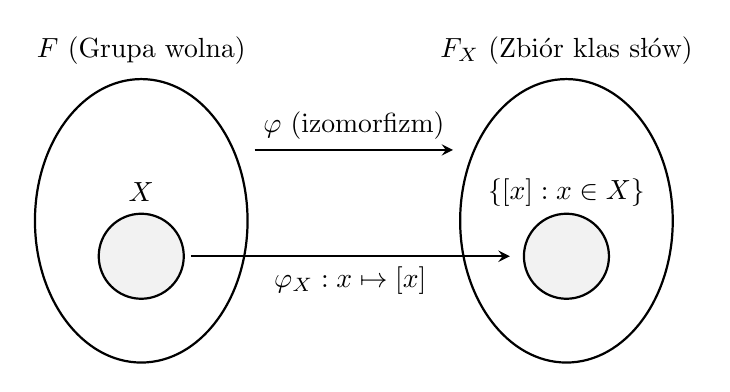
\begin{tikzpicture}[>=stealth, thick, scale=0.9]
    % --- LEWA STRONA: Abstrakcyjna grupa F ---
    \draw (0,0) ellipse (1.5cm and 2cm);
    \node at (0, 2.4) {$F$ (Grupa wolna)};
    
    % Zbiór X jako podzbiór
    \draw[fill=gray!10] (0, -0.5) circle (0.6cm);
    \node (X) at (0, 0.4) {$X$};

    % --- PRAWA STRONA: Model konstrukcyjny F_X ---
    \begin{scope}[xshift=6cm]
        \draw (0,0) ellipse (1.5cm and 2cm);
        \node at (0, 2.4) {$\mathbb{F}_{X}$ (Zbiór klas słów)};
        
        % Zbiór klas [X]
        \draw[fill=gray!10] (0, -0.5) circle (0.6cm);
	\node  at (0, 0.4) {$\{[x] : x \in X\}$};
    \end{scope}

    % --- ODWZOROWANIA ---
    % Izomorfizm grup
    \draw[->] (1.6, 1.0) -- (4.4, 1.0) node[midway, above] {$\varphi$ (izomorfizm)};
    
    % Bijekcja na poziomie generatorów
    \draw[->] (0.7, -0.5) -- (5.2, -0.5) node[midway, below] {$\varphi\restriction_{X}   : x \mapsto [x]$};
\end{tikzpicture}
\end{center}

\begin{remark}[Utożsamienie kanoniczne]
    Konstrukcja grupy $\mathbb{F}_X$ dostarcza modelu grupy wolnej, w której zbiorem generatorów jest zbiór klas słów jednoelementowych $\tilde{X} = \{ [x] : x \in X \}$. 
    
    Zauważmy, że odwzorowanie $j: X \to \mathbb{F}_X$ dane wzorem $j(x) = [x]$ jest iniekcją. Pozwala to na utożsamienie zbioru $X$ z jego obrazem $j(X) \subseteq \mathbb{F}_X$. W praktyce matematycznej, zamiast pracować na klasach $[x]$, dokonujemy „transportu struktury” na zbiór $F$, który zawiera wprost zbiór $X$.

\noindent Dzięki injektywności $j$, możemy zdefiniować strukturę grupy na zbiorze zawierającym $X$ tak, aby $X$ był jej \textbf{bazą}. Od tego momentu piszemy po prostu $X \subseteq F_X$, co jest drobnym, ale powszechnym nadużyciem oznaczeń upraszczającym rachunki.
\end{remark}

\begin{context}
    Od teraz przez $\mathbb{F}_X$ będziemy rozumieć \textbf{dowolną} grupę wolną o wolnym zbiorze generatorów $X$.
\end{context}

\subsection*{Charakteryzacje grup wolnych}

\begin{theorem}[Równoważne warunki]
    Dla $X \subseteq G$ następujące warunki są równoważne:
    \begin{enumerate}[label=\arabic*)]
        \item $G$ jest grupą wolną o wolnym zbiorze generatorów $X$.
        \item $G = \langle X \rangle$ oraz dwa słowa z $L_X$ definiują ten sam element $G$ wtedy i tylko wtedy, gdy są równoważne ($\sim$).
        \item $G = \langle X \rangle$ oraz słowo z $L_X$ definiuje $e_G$ wtedy i tylko wtedy, gdy jest równoważne słowu pustemu.
        \item $X$ jest \textbf{wolnym zbiorem generatorów}: $G = \langle X \rangle$ oraz każde niepuste słowo nieskracalne z $L_X$ definiuje element $\neq e_G$.
    \end{enumerate}
\end{theorem}
\begin{proof}
    TODO
\end{proof} 


\subsection*{Model słów zredukowanych}

\begin{definition}[Funkcja redukcji]
    Dla $u \in L_X$ oznaczamy przez $\rho(u)$ jedyne słowo nieskracalne w $[u]$.
\end{definition}

\begin{definition}[Grupa $N_X$]
    Niech $N_X$ oznacza zbiór słów nieskracalnych nad $X$. Definiujemy działanie:
    \[
    u \cdot v := \rho(uv) \quad \text{dla } u, v \in N_X.
    \]
\end{definition}

\begin{fact}
    $(N_X, \cdot)$ jest grupą izomorficzną z $\mathbb{F}_X$ przez izomorfizm $x \mapsto [x]$.
\end{fact}

\subsection*{Własność uniwersalna}

\begin{theorem}[Uniwersalność $\mathbb{F}_X$]
    Niech $H$ będzie grupą, $f: X \to H$ dowolną funkcją. Istnieje \textbf{jedyny} homomorfizm $\overline{f}: \mathbb{F}_X \to H$ przedłużający $f$.
    \[
    \begin{tikzcd}[row sep=30pt, column sep=30pt]
    X \arrow[dr, "\id"] \arrow[rr, "f"] & & H \\
    & \mathbb{F}_X \arrow[ur, "\exists ! \overline{f}"', dashed] &
    \end{tikzcd}
    \]
\end{theorem}
\begin{proof}
    TODO
\end{proof} 
\begin{theorem}[Charakteryzacja przez uniwersalność]
    Niech $X \subseteq G$, gdzie $G$ jest grupą. Jeśli para $(G, X)$ jest uniwersalna w sensie:
		\[
		    \left(\forall f: X\to H \right)\left(\exists ! \overline{f}:G\to H   \right)\left( f \subseteq \overline{f}   \right)    
		\]
    gdzie $H$ jest dowolną grupą, to istnieje izomorfizm $\varphi: G \overset{\cong}{\to} \mathbb{F}_X$ taki, że $\varphi\restriction_{X}   = \id_X$.
\end{theorem}
\begin{proof}
    TODO
\end{proof} 
\begin{corollary}
    Dla $X \subseteq G$ następujące warunki są równoważne:
    \begin{enumerate}[label=\arabic*)]
        \item $G$ jest grupą wolną o wolnym zbiorze generatorów $X$.
        \item $(G, X)$ jest uniwersalna w powyższym sensie.
    \end{enumerate}
\end{corollary}
\begin{proof}
    TODO
\end{proof} 
\begin{theorem}[O mocy generatorów]
    Jeśli $\mathbb{F}_X \cong \mathbb{F}_Y$, to $|X| = |Y|$.
\end{theorem}
\begin{proof}
    TODO
\end{proof} 
\subsection*{Przykłady i twierdzenia strukturalne}

\begin{enumerate}
    \item $\mathbb{Z} = \langle 1 \rangle \cong \mathbb{F}_1$.
    \item \textbf{Grupa ping-pongowa:}
    \[
    G = \left\langle 
    \begin{bmatrix} 1 & 2 \\ 0 & 1 \end{bmatrix},
    \begin{bmatrix} 1 & 0 \\ 2 & 1 \end{bmatrix}
    \right\rangle \le \mathrm{SL}_2(\mathbb{Z}) \cong \mathbb{F}_2.
    \]
\end{enumerate}

\begin{theorem}[Podgrupy wolne w $\mathbb{F}_2$]
    W grupie $\mathbb{F}_{\{x,y\}}$ podgrupa generowana przez $\{x^n y x^{-n} : n \in \mathbb{N}\}$(tutaj nie wiem czy nie miało być $x^{n}yz^{n}  $ ?) jest wolna o tych generatorach.
\end{theorem}
\begin{proof}
    TODO
\end{proof} 

\begin{corollary}[Hierarchia zanurzeń]
    Dla każdego $n \in \mathbb{N}$ istnieją monomorfizmy:
    \[
    \mathbb{F}_n \hookrightarrow \mathbb{F}_{\aleph_0} \hookrightarrow \mathbb{F}_2 \hookrightarrow \mathrm{SL}_2(\mathbb{R}).
    \]
\end{corollary}
\begin{proof}
    TODO
\end{proof} 
\begin{theorem}[Nielsen–Schreier]
    Podgrupa grupy wolnej jest wolna. Może mieć ona więcej generatorów.
\end{theorem}
\begin{proof}
    TODO
\end{proof} 
\begin{fact}
    Każda grupa $G$ jest obrazem homomorficznym pewnej grupy wolnej.
\end{fact}
\begin{proof}
    TODO
\end{proof} 
\subsection*{Prezentacje grup}

\begin{definition}[Prezentacja]
    Niech $X$ – zbiór, $A \subseteq \mathbb{F}_X$. \textbf{Prezentacją}
    \[
    \langle X \mid A \rangle := \mathbb{F}_X / \langle\!\langle A \rangle\!\rangle,
    \]
    gdzie $\langle\!\langle A \rangle\!\rangle$ – najmniejsza podgrupa normalna zawierająca $A$.
\end{definition}

\begin{intuition}
    Bierzemy grupę wolną $\mathbb{F}_X$ i „wymuszamy”, aby wszystkie słowa z $A$ (oraz ich konsekwencje) były równe jedności. Będzie to największa (uniwersalna) grupa spełniająca te relacje. Generowana przez warstwy elementów z $X$. 
\end{intuition}

\begin{remark}[Notacja]
    $\langle x_1,\dots,x_n \mid r_1,\dots,r_m \rangle$ oznacza $\langle \{x_1,\dots,x_n\} \mid \{r_1,\dots,r_m\} \rangle$.
\end{remark}

\begin{fact}[Uniwersalność prezentacji]
    Niech $G = \langle X \mid A \rangle$, $H$ – grupa, $f: X \to H$ taka, że $\overline{f}(a) = e_H$ dla każdego $a \in A$. Wtedy istnieje jedyny homomorfizm $\psi: G \to H$ przedłużający $f$.
\end{fact}

\begin{remark}
	Każda grupa ma prezentację, bo jest obrazem grupy wolnej
	\[
	G \cong \mfaktor{\mathbb{F}_{G}}{\langle \langle A \rangle  \rangle } = \langle G \mid A \rangle 
	.\] 
	gdzie $A = \{u \in \mathbb{F}_{G}: u \text{ wyliczone w } G = e_{G}\} $ oraz $\mfaktor{\mathbb{F}_{G}}{\langle \langle A \rangle  \rangle } = \mfaktor{\mathbb{F}_{G}}{A} $

	Tu $A = \ker(\overline{\id_{G}}) $, gdzie $\overline{\id_{G}}: \mathbb{F}_{G} \longrightarrow G$ 

	oraz $\overline{\id_{G}} \supseteq \id_{G}: G \to G$
\end{remark} 

\vspace{1em}

Istotne jest znajdowanie możliwie najprostszych prezentacji. Powyższa taka nie jest (za duże $X$ oraz za duże $A$ )

\subsection*{Przepis na znalezienie prezentacji}

Aby pokazać, że grupa $G$ ma prezentację $\langle x_1,\dots,x_n \mid r_1,\dots,r_m \rangle$:
\begin{enumerate}[label=\roman*)]
    \item Znajdź $g_1,\dots,g_n \in G$ takie, że $\langle g_1,\dots,g_n \rangle = G$.
    \item Sprawdź, że $g_i$ spełniają relacje $r_1,\dots,r_m$.
    \item Pokaż, że $|\langle x_1,\dots,x_n \mid r_1,\dots,r_m \rangle| \le |G|$.
\end{enumerate}

\subsection*{Przykłady prezentacji}

\begin{enumerate}
    \item $\mathbb{Z}_n \cong \langle x \mid x^n \rangle$.
    \item $\mathbb{Z}_2 \times \mathbb{Z}_2 \cong \langle x, y \mid x^2, y^2, [x,y] \rangle$.
    \item $S_3 \cong \langle x, y \mid x^2, y^3, xyxy \rangle$.
    \item $D_n \cong \langle x, y \mid x^2, y^n, xyxy \rangle$.
\end{enumerate}

\subsection*{Wolne grupy abelowe}

\begin{definition}[Wolna grupa abelowa]
    Grupa abelowa $A$ jest \textbf{wolną grupą abelową} o bazie $X \subseteq A$, jeśli dla dowolnej grupy abelowej $H$ i funkcji $f: X \to H$ istnieje \textbf{jedyny} homomorfizm $\overline{f}: A \to H$ przedłużający $f$. Czyli

    \[
	   	\left(\forall f : X \to H \right)\left(\exists ! \overline{f}: A \to H \right)\left( f \subseteq \overline{f} \right), \text{ gdzie } H \text{ grupa abelowa} .\]

	\[
		\begin{tikzcd}[row sep=30pt, column sep=30pt]
			X \arrow[dr, "\id"] \arrow[rr, "f"] & & H \\
			& A \arrow[ur, "\exists ! \overline{f}", dashed, hook] &
		\end{tikzcd}
	  \]
\end{definition}

\begin{remark}[Własności]
    \begin{enumerate}[label=\arabic*)]
						\item Dwie wolne grupy abelowe o bazach tej samej mocy są izomorficzne.
		\item Wolna grupa abelowa $X$ o bazie mocy $\kappa$ jest izomorficzna z $\mathbb{Z}^{\oplus\kappa}$
			 W szczególności gdy $\kappa < \aleph_0$ to dostajemy $\mathbb{Z}^{\kappa}$ 

        \item Wolna grupa abelowa o bazie mocy $\kappa$ jest izomorficzna z
        \[
        \mathbb{F}_{\kappa}^{\mathrm{ab}} := \mathbb{F}_\kappa / [\mathbb{F}_\kappa, \mathbb{F}_\kappa] \cong \langle \{x_i : i \in \kappa\} \mid x_i x_j x_i^{-1} x_j^{-1} \;(i \neq j) \rangle.
        \]
    \end{enumerate}
\end{remark}
\subsection*{Podsumowanie}

\begin{itemize}
    \item Grupa wolna $\mathbb{F}_X$ – „najogólniejsza” grupa generowana przez $X$ bez relacji.
    \item Charakteryzowana przez uniwersalność: dowolne przyporządkowanie generatorów do elementów dowolnej grupy rozszerza się do homomorfizmu.
    \item Każda grupa jest ilorazem grupy wolnej (ma prezentację $\langle X \mid R \rangle$).
    \item Twierdzenie Nielsen–Schreier: podgrupy grup wolnych są wolne.
    \item Wolne grupy abelowe to „przemienne” wersje grup wolnych – odpowiadają sumom prostym $\mathbb{Z}$.
\end{itemize}

\begin{intuition} 
 Grupa wolna to algebraiczny odpowiednik „swobodnego klejenia liter” – nie ma żadnych ograniczeń poza tymi, które muszą być (odwrotności, element neutralny). Prezentacje pozwalają opisać dowolną grupę przez generatory i relacje, podobnie jak baza i równania definiują przestrzeń liniową.
\end{intuition}
